\section{Conclusions}\label{sec:conclusion}

The durable contribution is the option cashflow and risk-accounting framework. A listed
option enters the allocation problem only after it has been represented as a premium-funded
cashflow, marked under a settlement convention, mapped into delta, gamma, vega, theta,
VIX-forward exposure, and residual risk, and forecast under the physical measure. Once
those objects exist, the Markowitz algebra is familiar: expected option cashflows and a
Greek-induced covariance matrix replace ordinary asset means and covariances.

The validation layer supports a coherent point-in-time research implementation, not
production tradability. Gross Sharpe, VIX hedge behavior, and option convexity are not
enough. They must survive premium accounting, exact settlement controls, post-cost
accounting at both the executable-cost and stress-cost layers, beta and Greek attribution,
inference with family-wise corrections, leave-one-out tests, cross-validation and
synthetic-universe robustness diagnostics, and no-lookahead checks. VIX options are useful in the framework because they are volatility
instruments rather than equity substitutes, but their expiry P\&L becomes headline-grade
only when exact VRO/SOQ settlement supports the rows being reported.

The trader's use case is a disciplined screening rule rather than an automatic trading
signal. A sleeve enters the book only when forecasted option premia survive premium cost,
spread, settlement, and Greek-budget checks. Convexity is worth paying for only when state
variables and hedge diagnostics justify the premium. Short option exposure is rejected or
capped when stress loss, assignment risk, liquidity, or margin screens dominate expected
carry. VIX options are treated as volatility instruments. When the validation layer cannot
separate option premia from equity drift, volatility carry, or optimistic execution, the
portfolio should sit in cash collateral, trade smaller, or use simpler diversifiers.

The breadth diagnostic adds a practical refinement. More names do not automatically save an
option-only optimizer; with the baseline historical-mean blend, the 56-name universe
mainly gives the inverse problem more noisy directions. Breadth begins to pay only after
the mean estimator is made structural-only and the liquidity model caps net contract
positions before trading. With VIX included, that combination moves the 57-group
\(\$1\) million book from \(-1.837\) to \(+1.499\) net Sharpe, with gross Sharpe
\(1.915\), while beating the best capped-naive book by \(1.232\) net Sharpe. Without VIX,
the 56-name optimizer reaches \(0.551\) net Sharpe, essentially tying capped equal-risk at
\(0.550\), so optimizer edge is not established. Even the positive VIX result is
small-account evidence. The locked E1 robustness layer strengthens but does not eliminate
the caveats: \texttt{larger+VIX} passes the resampled, refit, simulation, reality-check,
and rolling OOS screens most cleanly, while \texttt{larger} without VIX remains mixed and
\texttt{orig} without VIX is diagnostic because the hard-cap budget is below one NAV. In
the representative month-end contracts studied here, the cap budget supports roughly
\(\$1\)--\(\$2\) million of full deployment, not institutional scale.

\begin{figure}[H]
\centering
\IfFileExists{figures/final_breadth_validation_distributions.pdf}
  {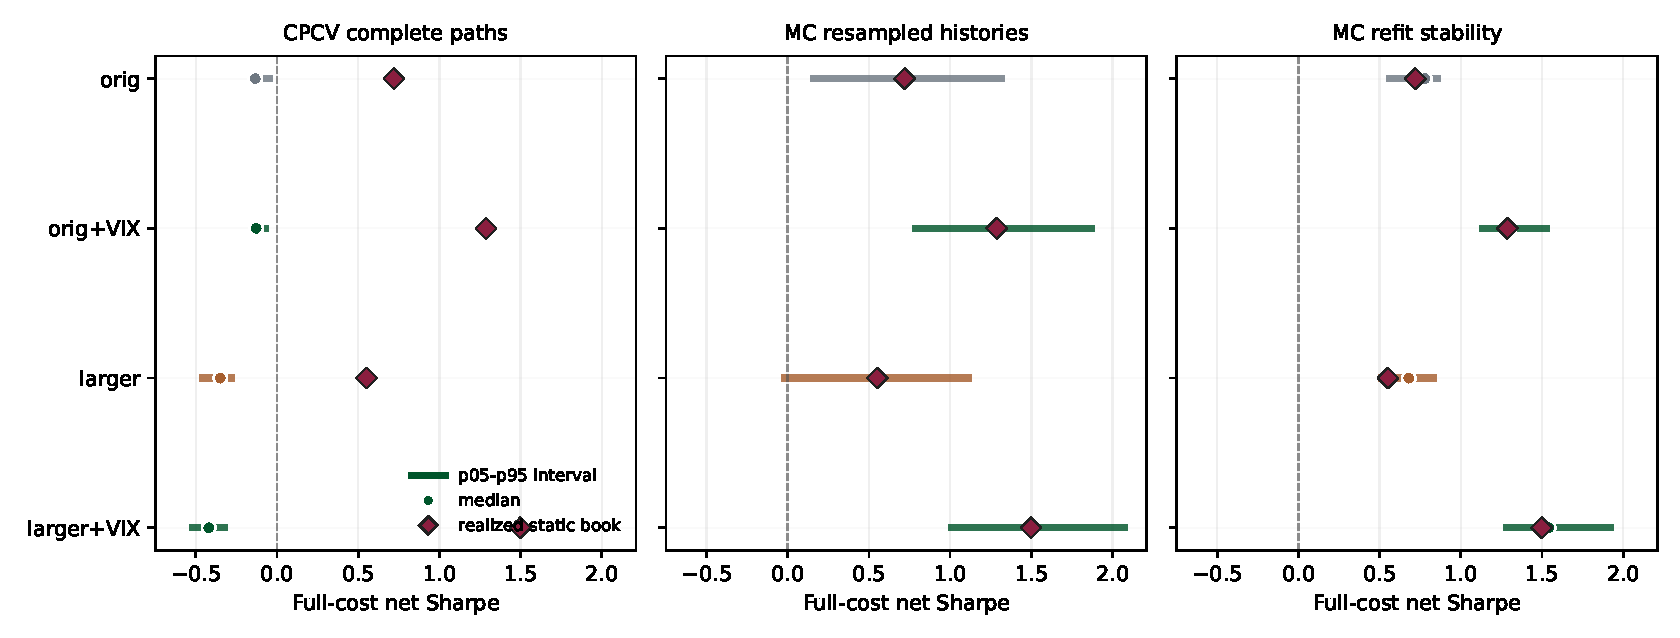
\includegraphics[width=\textwidth]{figures/final_breadth_validation_distributions.pdf}}
  {\fbox{\parbox{0.9\textwidth}{Run the final-results summary builder to render the
  validation-distribution figure.}}}
\caption{Final distributional validation for the four locked E1 configurations. Each
panel reports full-cost net Sharpe distributions for the locked E1 book: the horizontal
line is the 5th--95th percentile interval, the circle is the median, and the diamond is
the realized static \(\$1\) million book. CPCV complete paths are deliberately harsher
because they stitch short cost-timing windows; the Monte Carlo resampled and refit panels
show the stronger evidence for the VIX-enabled candidates.}
\label{fig:final_breadth_validation}
\end{figure}

\begin{figure}[H]
\centering
\IfFileExists{figures/final_baseline_comparison.pdf}
  {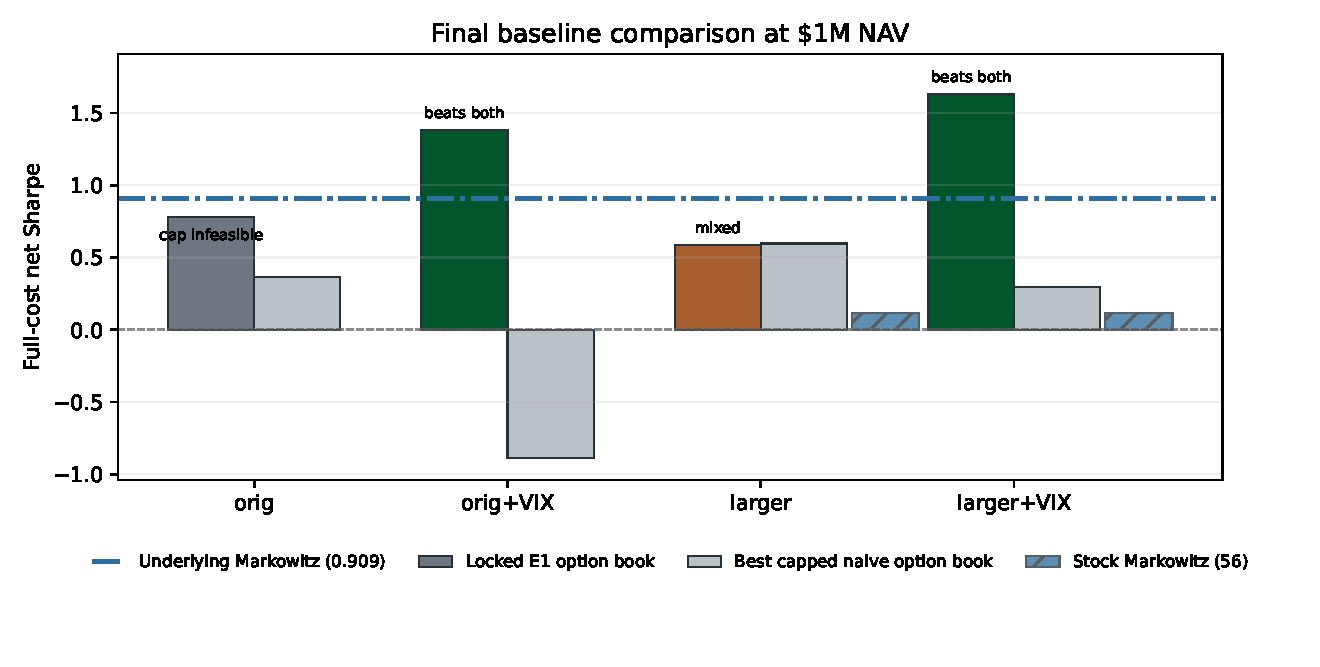
\includegraphics[width=0.94\textwidth]{figures/final_baseline_comparison.pdf}}
  {\fbox{\parbox{0.9\textwidth}{Run the final-results summary builder to render the
  baseline-comparison figure.}}}
\caption{Final baseline comparison. The stock baseline is the ordinary underlying
Markowitz portfolio on the same underlying equity universe. The naive option baseline is
the better of capped equal-premium and capped equal-risk option allocations for each
configuration. The VIX-enabled locked E1 books beat both baselines; the broad no-VIX book
essentially ties the naive option book and remains below stock Markowitz; the original
no-VIX row is diagnostic because full hard-cap deployment is infeasible.}
\label{fig:final_baseline_comparison}
\end{figure}

Figures~\ref{fig:final_breadth_validation} and~\ref{fig:final_baseline_comparison} are the
paper's final empirical scoreboard. The theory earns its strongest empirical support only
in the VIX-enabled books, where structural-only means, diagonal residual covariance,
\(N\)-scaled shrinkage, and net liquidity caps jointly beat both a regular stock
Markowitz baseline and naive capped option allocations. The no-VIX breadth result is
positive but not strong enough to claim optimizer edge, and the no-VIX eight-name result
is a capacity diagnostic rather than a deployable book.

This paper does not claim live-trading performance. The empirical sample is limited to the
available OPRA/Databento-derived equity-option panels, VIX option chains, monthly
snapshots, and exact VRO/SOQ coverage. Options execution, rates, margin, borrow,
assignment, and capacity are modeled through conservative research assumptions rather than
broker-level order and fill data. Production deployment would require richer quote
histories, executable bid/ask depth, broker margin previews, assignment and exercise
modeling, live routing, and reconciliation.

The immediate production-readiness step is forward shadow logging, not capital deployment.
Each rebalance should export the locked E1 target contracts, collect market-hours NBBO/CBBO
and displayed size, record marketable-limit fill assumptions, broker margin previews,
manual or automated rejections, and reconcile positions and cash. Those shadow ledgers can
reduce the execution caveat over time, but they remain shadow evidence until real broker
orders, fills, margin, exercise/assignment, and statements reconcile.

The conclusion is therefore deliberately restrained. Build the option cashflow. Charge the
premium and the implementation frictions. Estimate conditional premia before optimizing,
and turn noisy historical means off when \(T/n\) becomes thin. Constrain Greeks, beta, VIX
exposure, stress loss, and contract-level liquidity before trading, with caps on net
positions rather than split solver legs. Use regressions, attribution, regimes,
leave-one-out tests, breadth diagnostics, and inference to ask whether the result is more
than equity drift, volatility carry, estimator noise, or optimistic execution. Reject any
claim that depends on free options, future information, unpriced settlement, optimistic
costs, hidden short-option risk, or option depth that the market did not actually offer.
